%! TeX program = lualatex
%---------------------------ALLGEMEINE IMPORTS-------------------------------------
\documentclass[12pt,english,ngerman]{scrartcl}

\input{./input/shared_preamble.tex}
\lstloadlanguages{[ISO]C++}
\addbibresource{microcontroller.bib}
    % Kopfzeile
\ihead{SS22\\22.06.2022}
\chead{\textsc{Hinterleitner} Michael - 12002411 \\ \textsc{Philipp} Maximilian - 11839611}
\ohead{LU ECM-\\ Mikrocontroller}
    % Fußzeile
%--------------------------------------AB HIER DOKUMENT---------------------------------------------
\begin{document}
\includepdf{deckblatt5.pdf}
\tableofcontents
\newpage


%\section{Aufgabenstellung}\label{sec:Aufgabenstellung}

% Die nachfolgende Aufgabenstellung wurde von den Laborbetreuern bereitgestellt
% und beinhaltet sowohl Angaben zur Vorbereitung als auch zur praktischen
% Durchführung der Übung:

% zu 1: Aufgabenstellung Das vor der Übung verteilte Aufgabenblatt.
 \includepdf[
     pages=-,  % all pages
     addtotoc={
         1, section, 1, Aufgabenstellung, sec:Aufgabenstellung
     }
 ]{angabe.pdf}

% zu 2: Vorbereitung Es sind beide Vorbereitungen dem Protokoll beizufügen.
% \section{Vorbereitung}\label{sec:Vorbereitung}
%Die folgende Vorbereitung wurde vor der Laborübung 
 \includepdf[pages=-,
      addtotoc={
          1, section, 2, Vorbereitung, sec:Vorbereitung
      }]{./figures/ampel1.pdf}
 \includepdf[pages=-]{./figures/ampel2.pdf}
 \includepdf[pages=-]{./figures/game.pdf}


% zu 3: Grundlagen In den Grundlagen sollen die später verwendeten Formeln
% stehen und kurz erklärt werden, dabei ist es nicht notwendig Formeln
% herzuleiten. Quellenangaben sind an dieser Stelle von Vorteil, weil Sie so
% schnell die betreffenden Stellen in Unterlagen finden. In den Rechnungen
% werden grundlegende Annahmen skizziert und begründet und dann mit diesen
% Annahmen, die für die Schaltungen notwendigen Werte berechnet. Dabei kann
% auch gleich auf die später wirklich verwendeten Werte Bezug genommen werden -
% wir verwenden bei den Widerständen zum Beispiel von den Normwert-Reihen die
% E12 und/oder E24 Serie (nach DIN 41426 bzw. IEC 63).
\section{Grundlagen}\label{sec:Grundlagen}
Die Grundlage für diese Übung bietet die Plattform Arduino mit deren
Soft- und Hardware. Die Hardware, also das Mikrocontroller-Board (\textit{Arduino Uno R3}),
ist mitsamt der zugehörigen Pinbelegung in \autoref{sec:Aufgabenstellung}
(Aufgabenstellung) dargestellt. Neben der Rechenfunktion einer CPU,
was alleinstehend einem Mikroprozessor enstpricht, verfügt er wie andere
Mikrocontroller über weitere Elemente
wie Speicher respektive einem eigenen Schwingquarz zur Taktung,
was ihn zu einem kleinen, eigenständigen Computer macht.
Die integrierte Entwicklungsumgebung (IDE) der Arduino-Software erlaubt
freien Zugang (open-source). Die Ansteuerung des Boards über die IDE
erfolgt in einer C/C++ ähnlichen Programmiersprache.

Zur Auswertung sind keine Formeln notwendig, die in diesem Kapitel andererseits zu erwähnen
wären.
% zu 4: Versuchsdurchführung In diesem Punkt wird die Durchführung der
% einzelnen Aufgaben beschrieben. Im Simulationsteil ist die simulierte
% Schaltung mit allen Analyseparametern darzustellen. Im praktischen Teil sind
% die verwendete Geräte sowie die gemessenen Werte der verwendeten Bauteile
% anzugeben. Außerdem sind durchgeführte Funktionsüberprüfungen der Bauteile
% (Dioden, Transistor, etc.) anzuführen. Die Messergebnisse bzw. Oszillogramme
% sind mit Angabe der verwendeten Messgeräte anzugeben. Oszillogramme werden
% vom verwendeten Oszilloskop als Daten auf einen USB-Stick ausgegeben und
% können in das Protokoll aufgenommen werden. Das gleiche gilt für Schaltungen
% bzw. Ergebnissen von Simulationen. Es ist auf eine klare Darstellung der
% Messergebnisse und –auswertung zu achten (Tabellen, geeignete Grafiken). Die
% originalen, während des Versuchs angefertigten Aufzeichnungen sind dem
% Protokoll beizufügen. 
\section{Versuchsdurchführung}\label{sec:versuchsdurchfuehrung}
%Für den praktischen Teil an der Steckplatine wurden Widerstände der E12-Reihe,
%mit denen die in der Vorbereitung angegebenen respektive errechneten Werte
%angenähert wurden, verwendet.
%Da die exakten Komponenten für die logischen Gatter nicht in
%\textit{LTspice} zur Verfügung standen, wurden funktionstüchtig-äquivalente
%Bauteile in der Simulation verwendet. Die Gegenstücke in der Simulation wurden
%unten angeführt.
Die verwendeten Geräte sind \autoref{tab:geraeteliste} zu entnehmen.

\begin{table} [!h]
  \caption{Tabelle der verwendeten Geräte}
  \label{tab:geraeteliste}
  \centering
  \begin{tabular}{l|l}
    \hline
   \multicolumn{2}{ c }{\textbf{Geräteliste}} \\
    \hline
    \textbf{Gerät/Bauelement} & \textbf{Typ}\\
    \hline
    % Oszilloskop & \textit{Tektronix TDS 2002}\cite{oszilloscope}\\
    % Funktionsgenerator & \textit{H-TRONIC FG250D}\cite{funktionsgenerator} \\
    %Netzgerät & nicht bestimmbar\\
    %Multimeter & \textit{Fluke 175 TrueRMS}\cite{fluke175} \\
    % todo references
    %NOT-Gatter     &  \textit{74LS04}\cite{74LS04} & 74HCT04      \\
    %2x-NAND-Gatter &  \textit{74LS00}\cite{74LS00} & 74HCT00       \\
    Mikrocontroller-Board & \textit{Arduino Uno R3}  \\
    Widerstandsleiste &  \\
    7-Segment-Anzeige &  \\
    2x-NOR-Gatter & \textit{74LS02}\cite{74LS02}      \\ 
    %JK-MS-FF       &  \textit{74LS109}\cite{74LS109}      & 74HCT109  \\
    \hline
  \end{tabular}
\end{table}

\paragraph{Entprellter Schalter}\label{sec:schalter_aufbau}
%TODO text erklaeren wie der Schalter angesteuert wird und wo er verwendet wurde
Der entprellter Schalter wird als Signalgeber für die Schaltungen
verwendet. Der Aufbau dieses Schalters ist in
\autoref{fig:aufbau_schalter} ersichtlich, jedoch ist noch der \textit{GND} mit
Ground und \textit{VCC} mit \SI{5}{\volt} zu beschalten, damit das Signal von
den Schaltern für die jeweilige Betriebsart abgegriffen
werden kann.

Jeder dieser Schalter hat hierbei eine Standard-\textit{HIGH}- bzw.
\textit{LOW}-Betriebsart.

\begin{figure}[H]
  \centering
  \includegraphics[width=0.95\textwidth]{./figures/messungen/schalter.jpg}
  \caption{Dies sind die zwei entprellten Schalterplatinen mit je zwei Schalter
    ($S1$,$S2$) die entweder mit Standard-\textit{HIGH} oder -\textit{LOW} verwendet
    werden können. Diese werden durch Beschalten des \textit{GND} und der \SI{5}{\volt}
    Betriebsspannung in Betrieb genommen}
  \label{fig:aufbau_schalter}
\end{figure}

% dabei sollte man den schalter auf eingangs und Ausgangsspannungen ueber
% pruefen damit man sieht ob er fuer logische schaltung ueberhaupt brauchbar
% ist

% \paragraph{LED Leiste}
% %TODO text erklaeren wie der Leiste angesteuert wird und wo er verwendet wurde
% Damit die Eingangssignale und Ausgangssignale der logischen Schaltungen
% dargestellt werden können, wird eine LED-Leiste verwendet. Diese besteht aus
% mehreren LEDs mit Vorwiderständen und ist in \autoref{fig:aufbau_led} dargestellt und
% unterstützt bis zu 8 Aus- bzw. Eingangssignale. Die hier verwendete LED-Leiste
% hat einen Common-Ground und somit werden positiven Spannungssignale direkt an den
% verschiedenen Anschlüssen angelegt um die LED zum Leuchten zu bringen.

% \begin{figure}[H]
%   \centering
%   % \includegraphics[width=\textwidth, height=6cm,keepaspectratio]{./figures/messungen/ledleiste.jpg}
%   \caption{Dies ist die LED-Leiste, welche 8 LEDs mit je einem Vorwiderstand
%   hat. Sie ist in Common-Ground-Konfiguration und wird verwendet, um Signal
%   anzeigen zu können.}
%   \label{fig:aufbau_led}
% \end{figure}

% Damit die Aufnahmen der Schaltungen übersichtlich bleiben, wurden diese meistens
% von den Aufnahmen weggeschnitten und deren Funktion in der jeweiligen Grafik
% mittels \textit{LED} dargestellt oder in der Beschriftung gekennzeichnet bzw.
% erwähnt.


\subsection{Ampelschaltung}


% 2.1 Die Schaltung ist mit LTspice zu simulieren. Die Eingangspegel sowie die
% Ausgangspegel sind digital darzustellen  
\subsubsection{Simulation}

Da in der Vorbereitung der Programmablauf entworfen wurde, wurde
zunächst nur das Programm geschrieben und in der Simulationssoftware
\textit{SimulIDE} simuliert. Da die Funktionstüchtigkeit in der
Simulation gewährleistet wurde, konnte die Ampelschaltung aufgebaut
werden. In folgernder \autoref{fig:pap_ampel} ist der Programmablauf
nochmals ersichtlich. Des weiteren wurde der verwendete Code im Appendix
\ref{sec:code_ampel} hinzugefügt.

\begin{figure}[H]
  \centering
   \includegraphics[width=0.95\textwidth]{./figures/sim/papampel.pdf}
    \caption{Diese Grafik beinhaltet den Programmablauf einer, nach der
      \nameref{sec:Aufgabenstellung} entworfenen, Ampelschaltung mit
      einem Fußgängerübergang. Hier wurde der \textit{DIN 66001}
      verwendet, um den Programmablauf darzustellen. Falls der Plan
      zu klein ist, ist dieser in der \nameref{sec:Vorbereitung} nochmals größer ersichtlich.}
  \label{fig:pap_ampel}
\end{figure}

Beim Erstellen des Codes wurde auf die korrekte Beschaltung, wie in der
kleinen österreichischen Ampelkunde beschrieben, geachtet.

% 2.2 Das JK-Flipflop ist auf dem Steckboard aufzubauen und auf seine
% Funktionalität zu prüfen. Als Pegelgeber werden für das Steckboard vorhandene
% elektronisch entprellte Schalter verwendet. Die Ein- und Ausgangszustände sind
% durch LED´s anzuzeigen und die Funktionalität der Schaltung ist anhand
% ebendieser zu zeigen.  
% 2.3 Die Ergebnisse sind zu dokumentieren und zu diskutieren. 
\subsubsection{Steckboard}
% INSPIRATION
%TODO text
%Das Eingangssignal wurde durch einen entprellten Schalter, im Standardzustand
%\textit{LOW}, gegeben. Der Aufbau wird in \autoref{sec:schalter_aufbau} 
%dargestellt. Als Spannungsquelle wurde ein Netzgerät verwendet und auf \SI{5}{\volt}
%eingestellt. 

Die Schaltung ist mittels der \textit{SimulIDE} entworfen worden. In \autoref{fig:aufbau_skizze_ampel} 
ist der Aufbau der simulierten Schaltung ersichtlich. Die verwendeten
Widerstände sind in der Schaltung ersichtlich, wobei der Spannungsteiler
aus dem LDR und einem Pull-Down-Widerstand besteht.
%TODO figure
\begin{figure}[H]
  \centering
 \includegraphics[width=0.95\textwidth]{./figures/messungen/aufbau_ampel.png}
  \caption{Dies ist der skizzierte Aufbau der Ampelschaltung, welche in der \nameref{sec:Aufgabenstellung} beschrieben worden ist. }
  \label{fig:aufbau_skizze_ampel}
\end{figure}

Mit diesem als Vorbild wurde die eigentliche Schaltung aufgebaut.
Der Aufbau am Steckbrett ist in \autoref{fig:mess_wahrheitstabelle_jk} ersichtlich.
Die Spezifikationen der Schaltung können dieser entnommen werden.
%Um die Funktionstüchtigkeit des JK-MS-FF's zu überprüfen, wurde die
%Wahrheitstafel alle möglichen Schaltsignale der \textit{J K} Eingänge
%durchgeschaltet. Die Resultate sind in \autoref{fig:mess_wahrheitstabelle_jk}
%ersichtlich.
%TODO text messung
% Als  Pegelgeber wird  für  das  Steckboard  ein vorhandener  elektronisch
% entprellte  Schalter  (mit  Hilfe  eines RS-Flip-Flops)  verwendet.  Der
% Ein-  und Ausgangszustand  ist  jeweils durch  LEDs  anzuzeigen.  Die
% Funktionalität  der Schaltung ist anhand der LEDs zu zeigen.
%TODO figure messung

\begin{figure}[H]
  \centering
  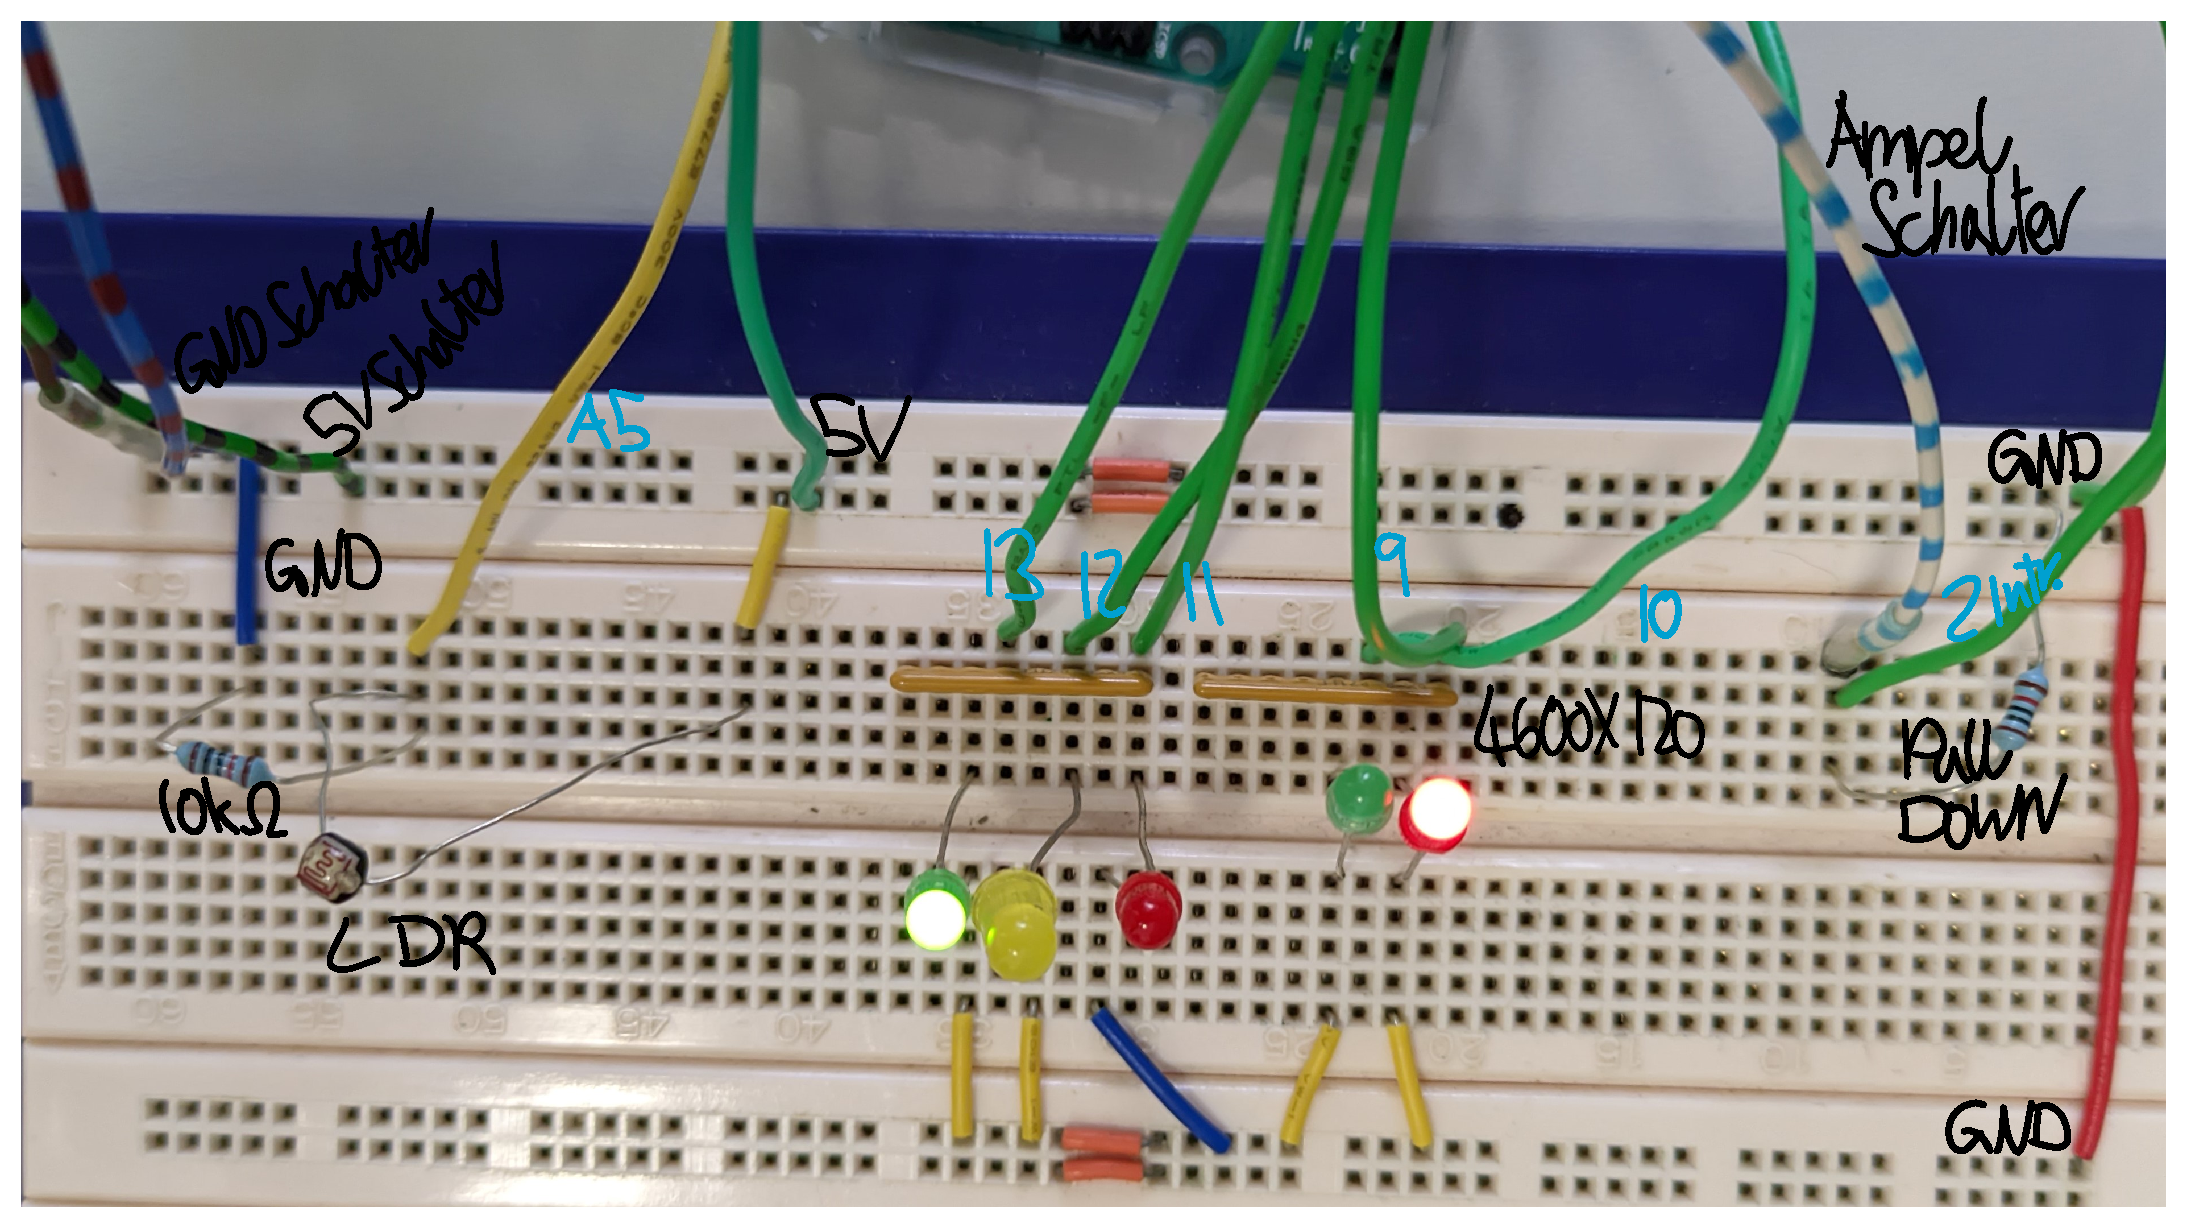
\includegraphics[width=0.95\textwidth]{./figures/messungen/mess_auf_ampel.pdf}
  \caption{Diese Abbildung beinhaltet den Aufbau am Steckbrett zur Ampelschaltung, wie in \autoref{fig:aufbau_skizze_ampel} ersichtlich.
  Die Beschriftungen in blau bezeichnen die am \textit{Arduino Uno R3} verwendeten
  Pins.}
\label{fig:mess_wahrheitstabelle_jk}
\end{figure}


% INSPIRATION
% \paragraph{Aufbau des CMOS-NAND-Gatters}
% Nun ist die CMOS-NOT Schaltung um zwei weitere MOSFETs erweitert worden, um ein
% NAND-Gatter zu bauen. Dies wurde wie in \autoref{fig:sim_aufbau_nand} aufgebaut.
% Es wurden, wie auch in \nameref{sec:mess_cmos}, entprellte Schalter als
% Pegelgeber und die LED-Leiste zur Visualisierung der Pegel (Signale) verwendet.
% Diese wurden ebenfalls an den geeigneten Abnahme-Stellen angeschlossen; wie diese genau
% angeschlossen wurden ist, der \autoref{fig:mess_aufbau_nand} entnehmbar.




\subsection{Reaktionsspiel}
% 2.1 Die Schaltung ist mit LTspice zu simulieren. Die Eingangspegel sowie die
% Ausgangspegel sind darzustellen. 
\subsubsection{Simulation}

Da in der Vorbereitung der Programmablauf entworfen wurde, wurde
zunächst nur das Programm geschrieben und in der Simulationssoftware
\textit{SimulIDE} simuliert. Da die Funktionstüchtigkeit in der
Simulation gewährleistet wurde, konnte das Reaktionsspiel aufgebaut
werden. In folgernder \autoref{fig:pap_game} ist der Programmablauf
nochmals ersichtlich. Des Weiteren wurde der verwendete Code im Appendix
\ref{sec:code_game} hinzugefügt.

\begin{figure}[H]
  \begin{center}
  \includegraphics[width=0.95\textwidth]{figures/sim/papgame.pdf}
  \end{center}
  \caption{Diese Grafik beinhaltet den Programmablauf eines, nach der
  \nameref{sec:Aufgabenstellung} entworfenen, Reaktionsspiels. Hier
  wurde der \textit{DIN 66001} verwendet, um den Programmablauf
  darzustellen. Falls dieser zu klein sein sollte, ist dieser in der \nameref{sec:Vorbereitung} nochmals größer ersichtlich.}
  \label{fig:pap_game}
\end{figure}


% 2.2 Die Schaltung ist am Steckboard aufzubauen und ihre Funktionalität zu
% zeigen (siehe Aufgabenstellung A). 
% 2.3 Die Ergebnisse sind zu dokumentieren und zu diskutieren. 
\subsubsection{Steckboard}
%Wie in \nameref{sec:Aufgabenstellung} gefordert, galt es eine Schaltung
%zu entwickeln, welche durch Anschlagen mindestens zweier Sensoren einen Alarm auslösen
%sollte. Diese Schaltung wurde, um die Fehlerquellen zu reduzieren, jedoch aus der
%Musterlösung entnommen und nicht die selbst Entworfene verwendet. Die vier
%Eingangsgrößen ($x1$, $x2$, $x3$, $x4$) wurden durch vier entprellte
%Schalter realisiert. Dabei sind $x1$ \& $x3$ im Standard \textit{LOW} und
%$x2$ \& $x4$ Standard \textit{HIGH} Betrieb geschaltet worden, damit die
%Alarmanlage bei Signalunterbrechung $x2$ \& $x4$ und einem Signal bei $x1$
%\& $x3$ anschlägt. Der Aufbau der Schaltung kann \nameref{fig:mess_aufbau_4bit}
%entnommen werden.

Die Schaltung ist mittels der \textit{SimulIDE} entworfen worden, in \autoref{fig:aufbau_skizze_game} 
ist der Aufbau der simulierten Schaltung ersichtlich. 
%TODO figure
\begin{figure}[H]
  \centering
 \includegraphics[width=0.95\textwidth]{./figures/messungen/aufbau_game.png}
  \caption{Dies ist der skizzierte Aufbau des Reaktionsspiels, welche in der \nameref{sec:Aufgabenstellung} beschrieben worden ist.}
  \label{fig:aufbau_skizze_game}
\end{figure}

Mit diesem als Vorbild wurde die eigentliche Schaltung aufgebaut.
Der Aufbau am Steckbrett ist in \autoref{fig:game_steckbrett} ersichtlich.
Die Spezifikationen der Schaltung können dieser ebenso entnommen werden.


Jedoch musste aus Verfügbarkeitsgründen ein NOR-Gatter statt einem OR-Gatter verwendet, 
wodurch im Code eine kleine Anpassung gemacht werden musste, dass nun mit 
einer \textit{FALLING-edge} statt einer \textit{RISING-edge} getriggert wurde. 
Dies ist im Code im \nameref{sec:Appendix} 
ersichtlich.

\begin{figure}[H]
  \begin{center}
  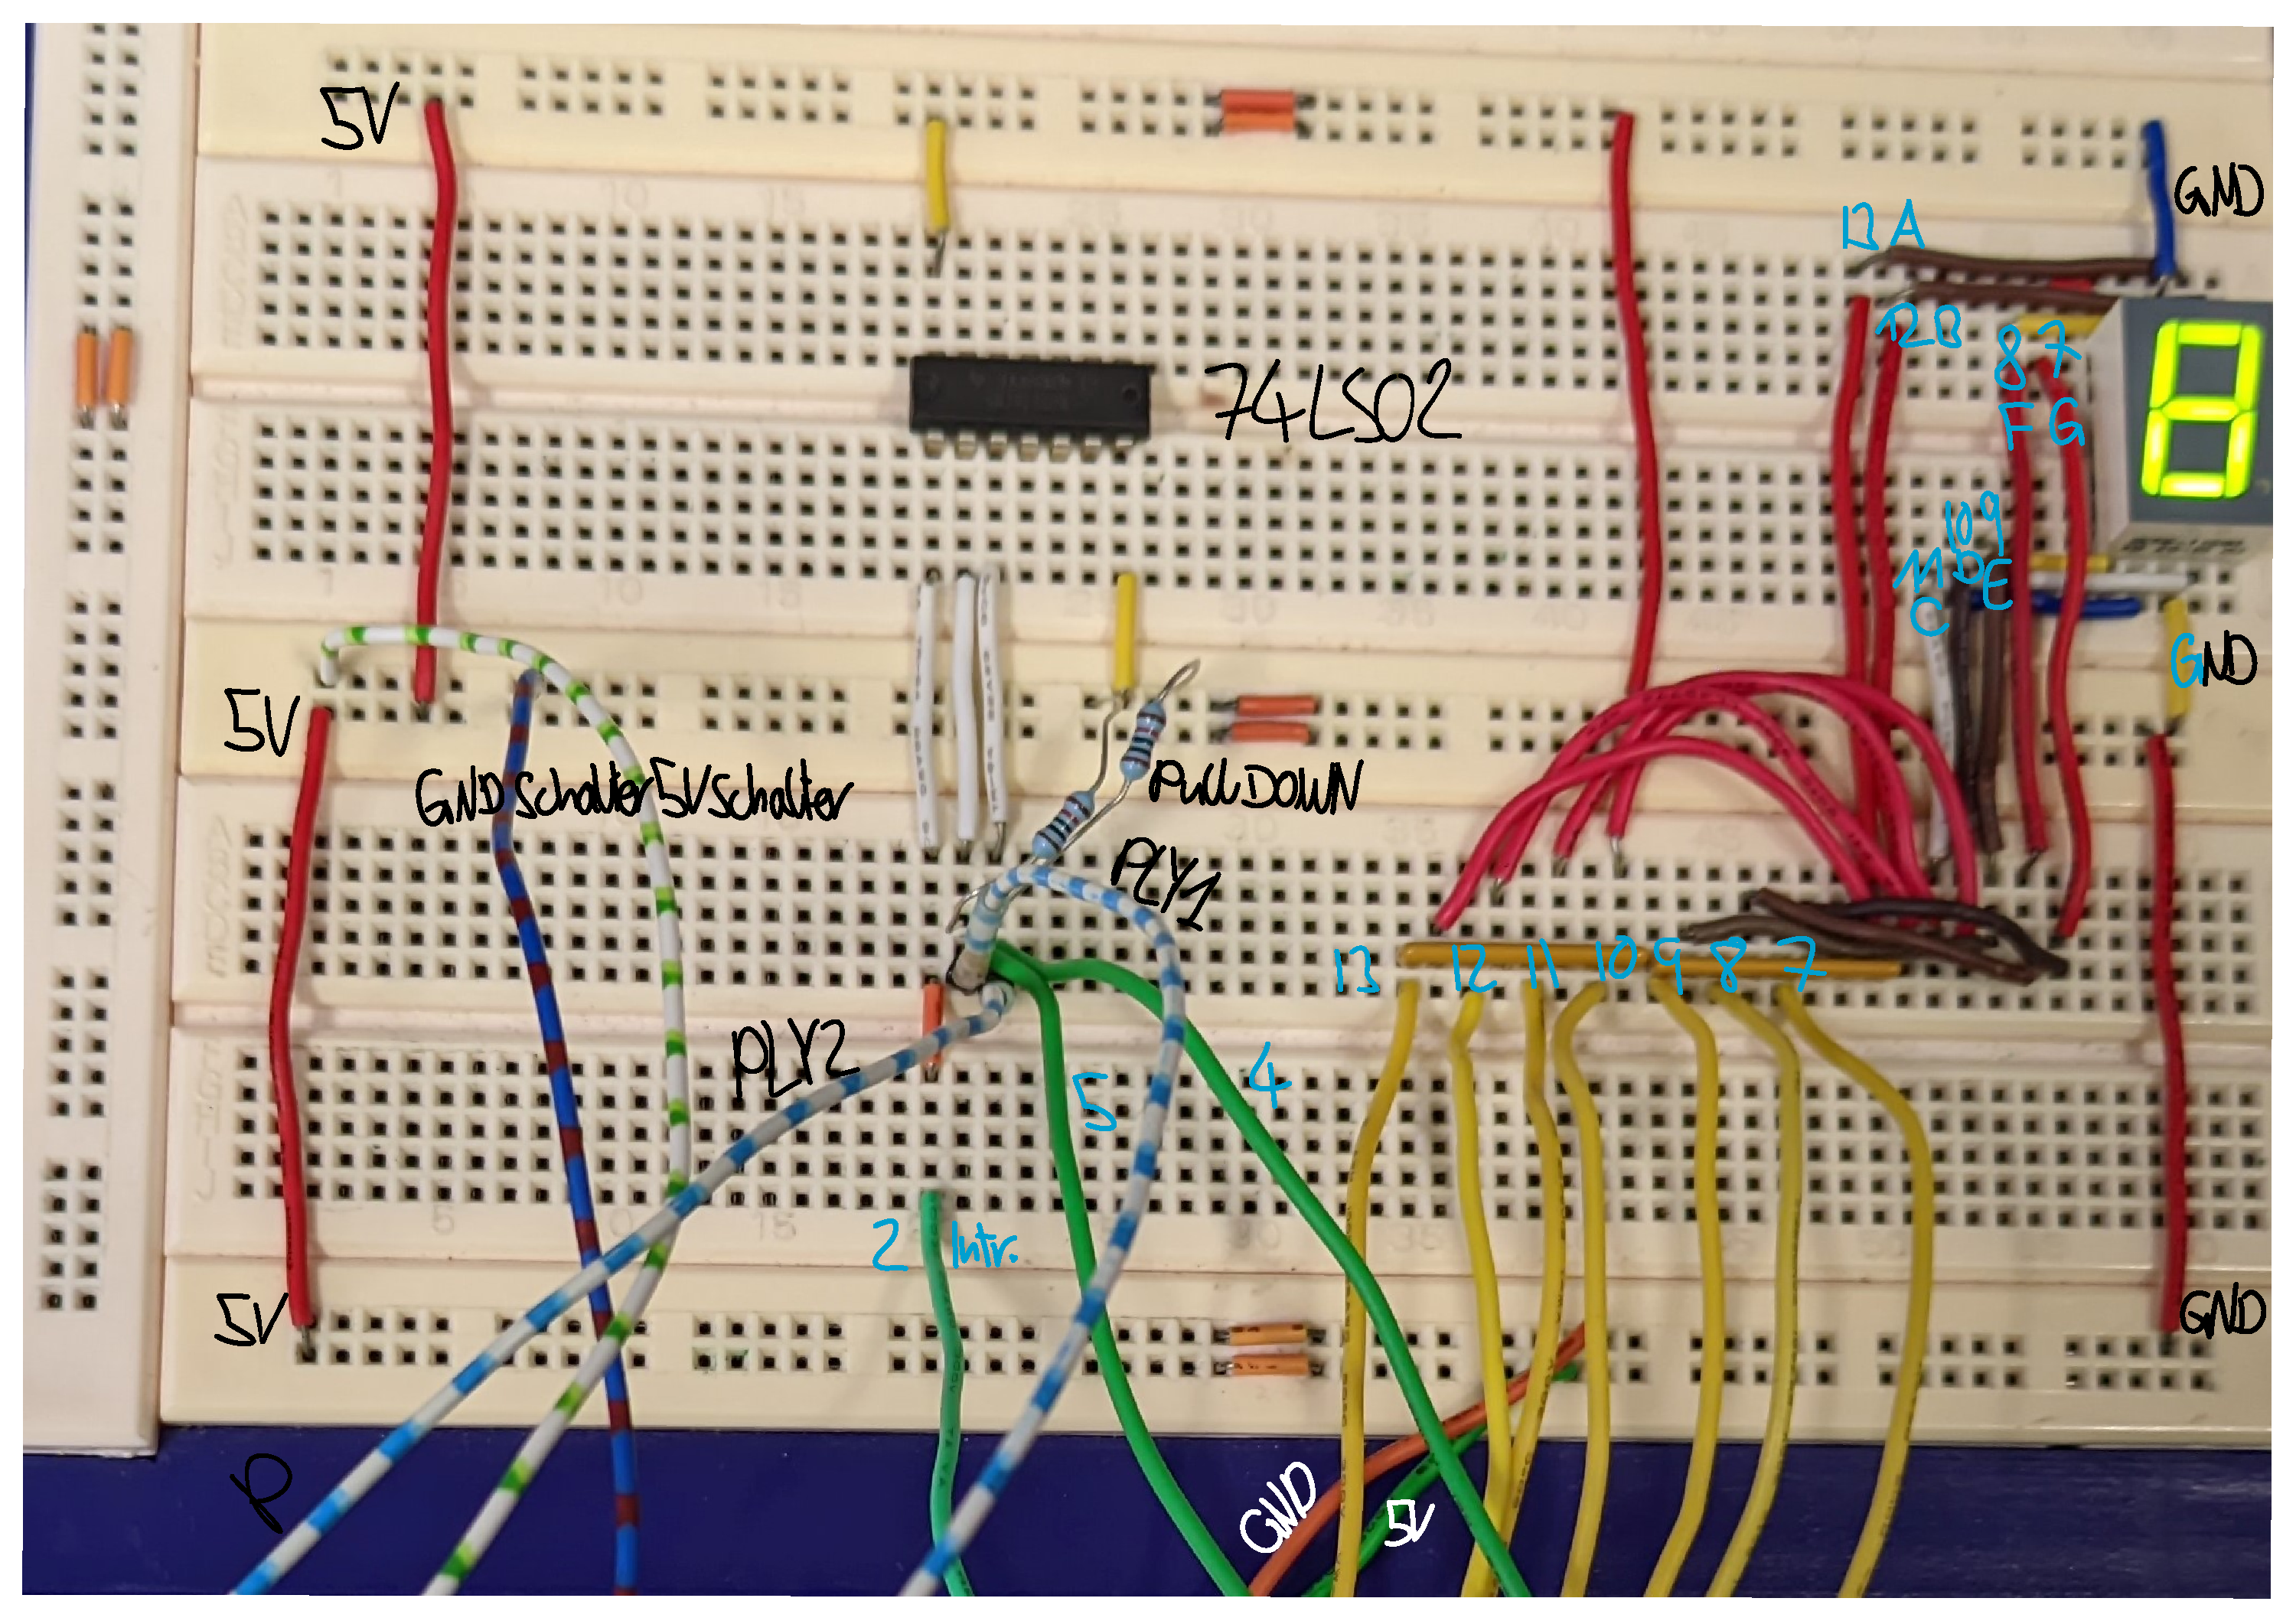
\includegraphics[width=0.95\textwidth]{figures/messungen/mess_auf_game.pdf}
  \end{center}
  \caption{Diese Abbildung beinhaltet den Aufbau am Steckbrett zum Reaktionsspiel, wie in \autoref{fig:aufbau_skizze_game} ersichtlich.
  Die Beschriftungen in blau bezeichnen die am \textit{Arduino Uno R3} verwendeten
  Pins.}
  \label{fig:game_steckbrett}
\end{figure}

% zu 4: Auswertung siehe EPM Skript nur Besprechung von Umformungen und 
% Sachen die man mit den Messungen machen muss damit man Conclusion und Wissen 
% gewinnen kann.
% Entsprechend der in Punkt 2. angegebenen Beziehungen (Formeln) ist aus den
% Messergebnissen in Punkt 5. das in Punkt 1. formulierte Endergebnis zu
% berechnen. Oft ist eine Ermittlung des Endergebnisses aus einer grafischen
% Darstellung bzw. eine grafische Veranschaulichung zweckmaßig. Dabei kann
% die Verwendung von Millimeterpapier oder Computerprogrammen hilfreich sein.
% Wenn eine Bearbeitung der Daten auf dem Computer erfolgt, sollte bei der
% Darstellung der Graphen eine sinnvolle Skalenteilung des Koordinatensystems
% gemacht werden. Die Unsicherheitsbetrachtung f ̈ur die angegebenen Messwerte,
% sowie fur Zwischen- und Endergebnisse ist in diesem Abschnitt
% nachvollziehbar zu beschreiben. Dabei ist nach Kapitel 1 vorzugehen und
% insbesondere auf die Klassifizierung der Unsicherheit (Typ-A/B) und die
% Unsicherheitsfortpflanzung einzugehen.
\section{Auswertung}\label{sec:Auswertung}
In diesem Protokoll ist keine Auswertung von Nöten, da die geforderten Resultate
direkt aus den Ergebnissen der Laborübung folgen. Die Funktionstüchtigkeit konnte 
festgestellt werden indem, dass Spiel gespielt wurde und die Ampelschaltung in Tag- und 
Nachtbetrieb verwendet worden ist. Das gewollte Verhalten wurde von den Betreuern bestätigt.
Hier sind Links zu Video der Schaltungen:
\href{https://www.dropbox.com/s/m3baaixz73scpv5/ampel.mp4?dl=0}{hier die Ampel} und 
\href{https://www.dropbox.com/s/5phbn6uqrtiq1w0/game.mp4?dl=0}{hier das Reaktionsspiel}.


% https://www.dropbox.com/s/m3baaixz73scpv5/ampel.mp4?dl=0
% https://www.dropbox.com/s/5phbn6uqrtiq1w0/game.mp4?dl=0

% zu 5: Diskussion und Zusammenfassung
% In der Zusammenfassung stehen noch einmal die wichtigsten Messergebnisse, wobei auf Tabellen und
% Abbildungen nur verwiesen werden soll. Die Ergebnisse sind auch zu diskutieren. Insbesondere müssen
% Abweichungen zwischen Simulation und praktischer Durchführung diskutiert werden.
\section{Diskussion und Zusammenfassung}\label{sec:Diskussion} 
\subsection{Diskussion}
Die Simulation in \textit{SimulIDE} wie auch der Aufbau am Steckbrett
haben den zu erwartenden Abläufen, die in \autoref{sec:Aufgabenstellung} (Aufgabenstellung)
gefordert sind, entsprochen.
%In \autoref{fig:sim_jk_wahrheit} von der Simulation und
%\autoref{fig:mess_wahrheitstabelle_jk}, welche die LEDs vom Steckbrett zeigt,
%ist das Verhalten eines CMOS-Inverters gut zu erkennen; dabei wird das Signal
%am Ausgang relativ zu jenem am Eingang negiert.
%Weiters ist anhand von \autoref{fig:sim_jk_wahrheit} aus der Simulation ersichtlich, dass
%der Schaltvorgang in CMOS endlich schnell erfolgt. Dabei ist ein deutliches
%Maximum des Stroms von \SI{4,21}{\milli \ampere} zu erkennen (siehe \autoref{fig:sim_inv_eingangsstrom}), 
%wenn (im Falle des Inverters) beide MOSFETs
%leitfähig sind, nämlich am Schnittpunkt der Spannungsverläufe.
%Die Spannung an diesen Schnittpunkten beträgt \SI{1,63}{\volt} 
%(siehe \autoref{fig:sim_inv_threshold}) und liegt
%somit innerhalb der für die Gate-Source-Spannung toleranten Intervalle
%von \SIrange{0.8}{2.4}{\volt} beim \textit{ZVN2106A} und von
%\SIrange{-3.5}{-1.5}{\volt} beim \textit{ZVP2106A} nach den zugehörigen Datenblättern.

%Das aus MOSFETs konstruierte NAND liefert als Ergebnis aller möglichen
%Kombinationen der beiden Eingangssignale \autoref{fig:sim_nand_wahrheit} für die Simulation
%und \autoref{fig:mess_wahrheitstabelle_nand} für die Steckbrettschaltung.
%Somit folgt der Verhalt jenem, der in der Wahrheitstabelle in \autoref{sec:Vorbereitung}
%(Vorbereitung) notiert wurde - der Ausgang ist stets \texttt{HIGH}, außer wenn
%beide Eingänge auf \texttt{High} sind.

%Genauso folgen für die Einbruchsicherungsschaltung \autoref{fig:sim_alarm_wahrheit} 
%und \autoref{fig:mess_wahrheitstabelle_alarm}
%der konstruierten Wahrheitstabelle in \autoref{sec:Vorbereitung} (Vorbereitung).
%Demnach löst der Alarm aus, sofern der \textit{Master-Switch} eingeschaltet ist, 
%wenn mindestens
%zwei Eingangsvariablen auf \texttt{HIGH} sind.


%Es wäre wohl vernünftiger gewesen, die Schaltung an der Steckplatine zunächst aufzubauen, um etwaige 
%Ungenauigkeiten durch die Widerstände 
\subsection{Zusammenfassung}
Im Rahmen dieser Laborübung wurden eine Ampelschaltung und ein Reaktionsspiel
mithilfe der Arduino-Plattform konzipiert, deren Funktionstüchtigkeit mit \textit{SimulIDE}
und am Steckbrett mit einem Arduino-Board verifiziert wurde.
%das Verhalten von einem CMOS-Inverter (siehe \autoref{fig:sim_jk_wahrheit}
%respektive \autoref{fig:mess_wahrheitstabelle_jk}), 
%einem aus CMOS konstruierten NAND (siehe \autoref{fig:sim_nand_wahrheit}
%respektive \autoref{fig:mess_wahrheitstabelle_nand}) und einer Einbruchsicherungsschaltung 
%(=Schaltnetz mit 4 Eingangsvariablen
%und \textit{Master-Switch}; siehe \autoref{fig:sim_alarm_wahrheit_aus}
%respektive \autoref{fig:mess_wahrheitstabelle_alarm}) erfolgreich mittels 
%Simulation und mithilfe von LEDs an Steckbrettschaltungen
%verifiziert.
\newpage
\section{Appendix}\label{sec:Appendix}
\subsection{Ampel Code}\label{sec:code_ampel}
\lstinputlisting[language={[ISO]C++}]{./ampel/ampel.ino}
%todo:put code in and remove comment
\subsection{Game Code}\label{sec:code_game}
\lstinputlisting[language={[ISO]C++}]{./game/game.ino}
%todo:put code in and remove comment
\newpage
\printbibliography

\listoffigures

\listoftables



\end{document}


